\chapter{Testes de Usabilidade}\label{chap:experimentos}\stepcounter{numchapters}

Neste capítulo são apresentados e discutidos os testes de usabilidade
utilizados para validar o software desenvolvido, apresentado no \autoref{chap:rsa}.
Este capítulo contempla o objetivo específico de validar o sistema desenvolvido.

\section{Teste de Usabilidade}

Um dos requisitos do software apresentado no \autoref{chap:software}, \autoref{sec:requisitos} era que:
\begin{description}
\item[Facilidade do uso e de criação de votação:] O sistema não deve oferecer
dificuldades de uso e de criação de questões;
\end{description}

Ou seja, trata-se um de um requisito não funcional do tipo produto (requisitos que
especificam o comportamento do produto), mais especificamente um requisito de usabilidade.
A usabilidade propõe-se a garantir que o produto seja fácil de aprender a usar, eficaz e
agradáveis do ponto de vista do usuário \cite{rogers2013design}.
Para \citeonline{nielsen_2012}, a usabilidade é definida por cinco componentes de qualidade:

\begin{description}
  \item[Apreensibilidade (\textit{Learnability}):] facilidade para os usuários realizarem tarefas básicas
  pela primeira vez.
  \item[Eficiência (\textit{Efficiency}):] rapidez com que os usuários realizam uma tarefa, uma vez aprendida.
  \item[Recordação (\textit{Memorability}):] facilidade em lembrar como fazer algo novamente, depois de um período sem uso.
  \item[Erros (\textit{Errors}):] o sistema deve ter uma baixa taxa de erros e ter capacidade de
  recuperação dos erros.
  \item[Satisfação (\textit{Satisfaction}):] quão agradável é utilizar o sistema.
\end{description}

\subsection{Métodos, tarefas e usuários}

Para verificar a usabilidade do software desenvolvido, realizou-se testes de usabilidade, com o
objetivo de testar o quão usável é o software. Para isso, utilizou-se o seguinte método: teste de usabilidade
que incluía a observação dos usuário utilizando o software e também a gravação em vídeo da tela do
software. Além disso, um questionário de satisfação SUS\nomenclature{SUS}{System Usability Scale} (\textit{System Usability Scale}) do usuário foi utilizado para descobrir como
os usuários se sentiram usando o software.

\subsection{Questionário de satisfação: SUS}\label{sub:sus}

O SUS é um método normalizado desenvolvido em 1986 por John Brooke.
Ele é um questionário constituído por apenas 10 itens, gratuito e simples de usar.
Utiliza-se a escala de Likert (valores 1 - \textit{discordo totalmente} e 5 \textit{concordo totalmente})
O critérios que o SUS ajuda a avaliar são \cite{brooke1996sus}:

\begin{description}
  \item[Efetividade (\textit{effectiveness})] a capacidade dos usuários de completar tarefas.
  \item[Eficiência (\textit{efficiency})] o nível de esforço e recursos necessários completar as tarefas.
  \item[Satisfação (\textit{satisfaction})] reações subjetivas dos usuários (a experiência foi satisfatória?).
\end{description}

O questionário SUS foi originalmente escrito na língua inglesa. Dessa forma, a versão para língua portuguesa
utilizada nesse trabalho (disponível no \autoref{appendix:sus}) foi a desenvolvida por \citeonline{tenorio2010desenvolvimento} que passou por um processo
de tradução.

O resultado do SUS é a soma individual de cada item, resultando em um número entre 0 e 100.
Para os itens 1, 3, 5, 7 e 9 deve-se subtrair 1 de cada resposta. Para os itens 2, 4, 6, 8 e 10 deve-se
subtrair de 5 o valor de cada resposta. O escore final SUS é soma de todos os itens multiplicada por 2,5 \cite{brooke1996sus}.

\subsection{Tarefas}

As tarefas foram desenvolvidas de modo a permitir que os participantes
percorressem todo o processo para permitir disponibilizar as questões para os alunos,
consistindo basicamente nas seguintes tarefas: cadastrar uma turma e alunos, criar questões, iniciar uma sessão de questões,
e controlar a sessão de questões. As tarefas foram escritas no seguinte formato:

\begin{description}
  \item[Título:] em poucas palavras o objetivo da tarefa.
  \item[Descrição:] contexto da tarefa (situação para realizar a tarefa).
  \item[Tarefas:] o que o participante deveria fazer.
\end{description}

O exemplo da \autoref{fig:usabilidade_teste} exibe uma tarefa apresentada para
os participantes seguindo o formato apresentado. A lista completa e detalhada das tarefas
utilizadas no teste está disponível no \autoref{appendix:tasks}.

\begin{figure}[!ht]
  \centering
  \caption{Exemplo de uma tarefa do teste de usabiliade}
  \label{fig:usabilidade_teste}
  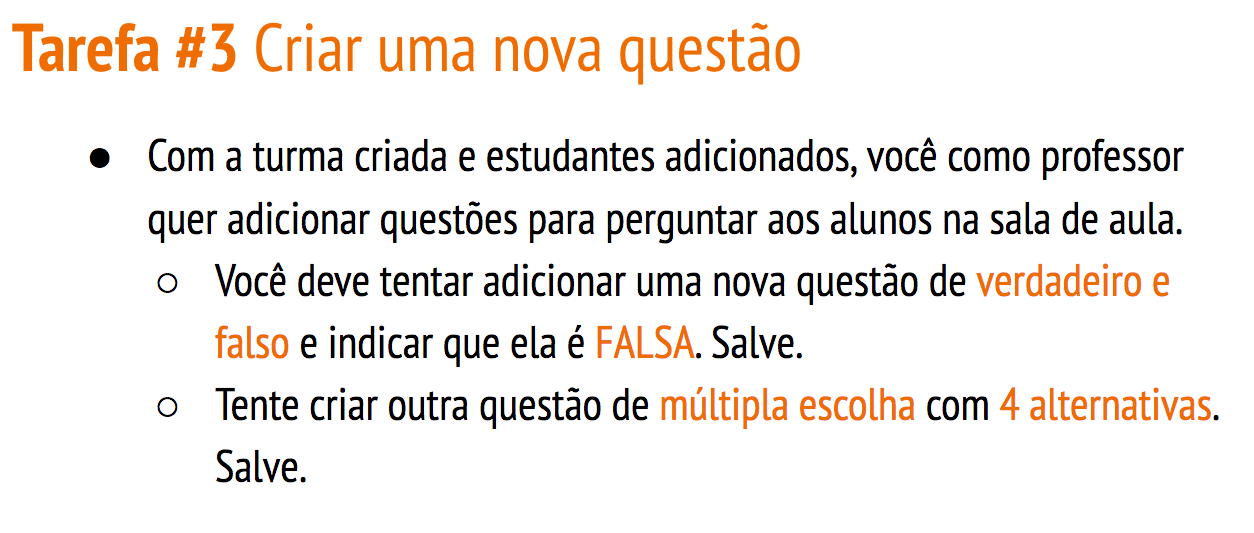
\includegraphics[scale=0.35]{imagens/usability_task}
  \doautor
\end{figure}
% \clearpage

A seguir, apresenta-se quais ações eram pretendidas dos participantes em cada tarefa:
\begin{enumerate}[label={},leftmargin=*]
  \item \textbf{Tarefa \#1 Criar uma nova turma}
  \begin{itemize}
    \item Espera-se que o professor identifique facilmente a opção para adicionar uma turma e habilite
    a opção para ativar a turma que ele criou.
  \end{itemize}

  \item \textbf{Tarefa \#2 Adicionar estudantes em uma turma}
  \begin{itemize}
    \item Espera-se que o professor identifique o botão para adicionar estudantes. Na tela de adicionar
    estudantes, que ele identifique a opção \textit{Adicionar manualmente}, adicione os estudantes e em seguida
    salve as alterações.
  \end{itemize}

  \item \textbf{Tarefa \#3 Criar uma nova questão}
  \begin{itemize}
    \item Espera-se que o professor localize a aba \textit{Questões} e identifique facilmente
    o botão para adicionar uma questão. No formulário para adicionar uma questão, que ele
    adicione a pergunta, alternativas e marque uma opção como correta.
  \end{itemize}

  \item \textbf{Tarefa \#4 Realizar frequência dos estudantes}
  \begin{itemize}
    \item Nessa tarefa, o botão de frequência está na aba \textit{Aula}. Seguindo as tarefas de forma
    sequencial, o professor estará na aba \textit{Questões}. Nesse sentido, espera-se
    que o professor explore a aba \textit{Aula} e identifique o botão \textit{Frequência}.
  \end{itemize}

  \item \textbf{Tarefa \#5 Acessar a sala como estudante}
  \begin{itemize}
    \item Agora no papel de aluno, espera-se que o professor relacione o código da turma que
    ele criou na tarefa 1 para ter acesso como estudante no aplicativo. Na tela de identificação do estudante,
    espera-se que ao ler a mensagem ele coloque o código de identificação de um estudante adicionado na tarefa 2.
  \end{itemize}

  \item \textbf{Tarefa \#6 Responder a frequência}
  \begin{itemize}
    \item Já identificado no aplicativo do estudante, espera-se que o professor identifique
    o botão \textit{Responder chamada} e entre com o código gerado para a frequência na tarefa 4.
    Por último, espera-se que ele verifique que no software do professor, o sistema identificou
    que um aluno realizou a frequência.
  \end{itemize}

  \item \textbf{Tarefa \#7 Iniciar sessão de perguntas}
  \begin{itemize}
    \item  Espera-se que o professor navegue para a aba \textit{Questões} e identifique
    que para iniciar uma sessão de perguntas, ele deve selecionar pelo menos uma questão que ele criou
    na tarefa 3. Ele também deve explorar as opções de controle da sessão e ativar uma questão para votação.
  \end{itemize}

  \item \textbf{Tarefa \#8 Responder questão}
  \begin{itemize}
    \item Com a questão já ativada, o professor deve facilmente escolher uma alternativa e
    enviar a resposta utilizando o aplicativo do estudante.
  \end{itemize}

  \item \textbf{Tarefa \#9 Finalizar sessão de perguntas}
  \begin{itemize}
    \item Espera-se que o professor explore as opções de pausar, mostrar a resposta correta e mostrar
    o resultado da votação.
  \end{itemize}

  \item \textbf{Tarefa \#10 Encerrar sessão de perguntas}
  \begin{itemize}
    \item Espera-se que o professor identifique a opção de encerrar a sessão de perguntas.
  \end{itemize}

  \item \textbf{Tarefa \#11 Verificar resposta dos estudantes}
  \begin{itemize}
    \item Encerrando a sessão de perguntas, a sessão encerrada deve ser listada no software.
    Espera-se que o professor clique na opção detalhes da sessão listada e explore as respostas dos estudantes.
  \end{itemize}
\end{enumerate}

\subsection{Usuários}

Os participantes foram considerados usuários típicos, 4 professores da UNIVASF e
um estudante de graduação de que já trabalhou como professor do ensino médio. Todos os
participantes eram do sexo masculino.

\subsection{Resultado e discussões}

Com a utilização do questionário SUS foi possível mensurar o grau de satisfação quanto
a usabilidade do software desenvolvido. Além disso, ele permite avaliar os componentes da
qualidade indicadas por \citeonline{nielsen_2012} distribuídas nas afirmativas do questionário:

\begin{itemize}
  \item \textbf{Apreensibilidade}: afirmações 3, 4, 7 e 10:
  \begin{itemize}
    \item AF3: Eu achei o sistema fácil de usar.
    \item AF4: Eu acho que precisaria de ajuda de uma pessoa com conhecimentos
    técnicos para usar o sistema
    \item AF7: Eu imagino que as pessoas aprenderão como usar esse sistema
    rapidamente.
    \item AF10: Eu precisei aprender várias coisas novas antes de conseguir
    usar o sistema.
  \end{itemize}
  \item \textbf{Eficiência}: afirmações 5, 6 e 8:
  \begin{itemize}
    \item AF5: Eu acho que as várias funções do sistema estão muito bem
    integradas.
    \item AF6: Eu acho que o sistema apresenta muita inconsistência.
    \item AF8: Eu achei o sistema atrapalhado de usar.
  \end{itemize}
  \item \textbf{Recordação}: afirmação 2:
  \begin{itemize}
    \item AF2: Eu acho o sistema desnecessariamente complexo.
  \end{itemize}
  \item \textbf{Erros}: afirmação 6:
  \begin{itemize}
    \item AF6: Eu acho que o sistema apresenta muita inconsistência.
  \end{itemize}
  \item \textbf{Satisfação}: afirmações 1, 4 e 9:
  \begin{itemize}
    \item AF1: Eu acho que gostaria de usar esse sistema frequentemente.
    \item AF4: Eu acho que precisaria de ajuda de uma pessoa com conhecimentos
    técnicos para usar o sistema.
    \item AF9: Eu me senti confiante ao usar o sistema.
  \end{itemize}
\end{itemize}

A \autoref{tab:sus_result} apresenta as respostas dos 5 participantes no teste de usabilidade.
A coluna \textit{Afirmações} contém as afirmações do questionário SUS, seguida pelas colunas
\textit{P1,$\ldots$,P5}, que representam cada participante. Os valores da escala de Likert
(1 - discordo totalmente e 5 - concordo plenamente) escolhidas pelos participantes estão mostradas
na tabela.

Abaixo das afirmações apresenta-se a \textit{Pontuação SUS} de cada questionário. O cálculo
para obter tais resultados foi apresentado na \autoref{sub:sus}. Obteve-se uma média de
85,50 com desvio padrão de 9,42.

A \autoref{fig:sus_score} apresenta como alguns estudos classificam a nota média do SUS.
Dessa forma, o software pode ser classificado como \textit{80-90, aceitável, B e Excelente}.
Assim, pode-se dizer que o software apresenta os cinco componentes de qualidade de usabilidade definidos
por \citeonline{nielsen_2012}, ou seja, apreensibilidade, eficiência, recordação, erros e satisfação
de forma excelente.

\begin{figure}[!ht]
  \centering
  \caption{Resultado do questionário SUS}
  \label{tab:sus_result}
\begin{tabular}{>{\raggedright}p{0.45\paperwidth}||ccccc}
\hline
\multicolumn{6}{c}{\textbf{Resultado do questionário SUS}}\tabularnewline
\hline
\hline
\multirow{2}{0.5\paperwidth}{\centering{}\textbf{Afirmações}} & \multicolumn{5}{c}{Participantes}\tabularnewline
 & P1 & P2 & P3 & P4 & P5\tabularnewline
\hline
\hline
\textbf{AF1} - {\small{}Eu acho que gostaria de usar esse sistema frequentemente.}
 & 5 & 4 & 4 & 4 & 5\tabularnewline
\textbf{AF2} - {\small{}Eu acho o sistema desnecessariamente complexo.}
 & 4 & 1 & 2 & 2 & 1\tabularnewline
\textbf{AF3} - {\small{}Eu achei o sistema fácil de usar.}
 & 4 & 5 & 3 & 4 & 5\tabularnewline
\textbf{AF4} - {\small{}Eu acho que precisaria de ajuda de uma pessoa com conhecimentos
técnicos para usar o sistema.}
 & 1 & 1 & 4 & 4 & 2\tabularnewline
\textbf{AF5} - {\small{}Eu acho que as várias funções do sistema estão muito bem
integradas.}
 & 4 & 5 & 5 & 4 & 4\tabularnewline
\textbf{AF6} - {\small{}Eu acho que o sistema apresenta muita inconsistência.}
 & 2 & 1 & 1 & 1 & 1\tabularnewline
\textbf{AF7} - {\small{}Eu imagino que as pessoas aprenderão como usar esse sistema
rapidamente.}
 & 5 & 5 & 4 & 4 & 5\tabularnewline
\textbf{AF8} - {\small{}Eu achei o sistema atrapalhado de usar.}
 & 1 & 1 & 1 & 2 & 1\tabularnewline
\textbf{AF9} - {\small{}Eu me senti confiante ao usar o sistema.}
 & 5 & 4 & 4 & 5 & 5\tabularnewline
\textbf{AF10} - {\small{}Eu precisei aprender várias coisas novas antes de conseguir
usar o sistema.}
 & 1 & 2 & 2 & 1 & 1\tabularnewline
\hline
\centering{}\textbf{Pontuação SUS} & 85 & 95 & 75 & 77,5 & 95\tabularnewline
\hline
\end{tabular}
\doautor
\end{figure}

\begin{figure}[!ht]
  \centering
  \caption{Comparação das classificações adjetivas, pontuações de aceitabilidade e escalas de classificação escolar, em relação ao escore médio do SUS}
  \label{fig:sus_score}
  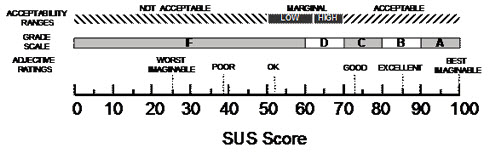
\includegraphics[scale=1.5]{imagens/sus_score}
  \fonte{\cite{bangor2009determining}}
\end{figure}

\clearpage
\subsubsection{Análise das gravações por tarefa}
Para cada uma das tarefas propostas, as principais observações de cada tarefa
estão descritas a seguir:

\begin{enumerate}[label={},leftmargin=*]
  \item \textbf{Tarefa \#1 Criar uma nova turma}
  \begin{description}
    \item [Expectativa:] Espera-se que o professor identifique facilmente a opção para adicionar uma turma e habilite
    a opção para ativar a turma que ele criou.
    \item [Observações:] Todos os participantes conseguiram concluir essa tarefa sem ajuda. O botão
    para adicionar a turma foi identificado com facilidade. 1 participante não ativou a turma.
    \item [Melhorias:] Quando nenhuma turma estiver ativada, exibir uma mensagem indicando:
    \textit{Você ainda não tem uma turma ativada. Ative uma turma para iniciar uma sessão de perguntas}.
    Outra solução seria ativar a primeira turma criada automaticamente e exibir uma mensagem para o usuário.
  \end{description}

  \item \textbf{Tarefa \#2 Adicionar estudantes em uma turma}
  \begin{description}
    \item [Esperado:] Espera-se que o professor identifique o botão para adicionar estudantes. Na tela de adicionar
    estudantes, que ele identifique a opção \textit{Adicionar manualmente}, adicione os estudantes e em seguida
    salve as alterações.
    \item [Observações:] 2 participantes tiveram dificuldades para encontrar o botão para
    adicionar estudantes no canto inferior direito da tela.
    \item [Solução:] Quando a lista de estudantes estiver vazia, exibir uma mensagem indicando:
    \textit{Você ainda não tem nenhum estudante cadastrado na turma. Comece adicionando estudantes nas opções ao lado.}
  \end{description}

  \item \textbf{Tarefa \#3 Criar uma nova questão}
  \begin{description}
    \item [Esperado:] Espera-se que o professor localize a aba \textit{Questões} e identifique facilmente
    o botão para adicionar uma questão. No formulário para adicionar uma questão, que ele
    adicione a pergunta, alternativas e marque uma opção como correta.
    \item[Observações:] Todos os participantes concluíram essa tarefa sem ajuda. 2 participantes
    tiveram um pouco de dificuldade para marcar uma alternativa como correta.
    \item[Melhorias:]
    Colocar a descrição \textit{Correta} ao lado do botão que seleciona a questão como correta.
    Outra melhoria seria que quando o tipo de questão for de múltipla escolha, já adicionar
    duas alternativas como padrão, diminuindo assim dois cliques no processo.
  \end{description}

  \item \textbf{Tarefa \#5 Acessar a sala como estudante}
  \begin{description}
    \item [Esperado:] Agora no papel de aluno, espera-se que o professor relacione o código da turma que
    ele criou na tarefa 1 para ter acesso como estudante no aplicativo. Na tela de identificação do estudante,
    espera-se que ao ler a mensagem ele coloque o código de identificação de um estudante adicionado na tarefa 2.
    \item [Observações:] 1 participante precisou de ajuda para completar a tarefa. Uma observação de um
    participante foi que ele estava precisando digitar o código da turma a todo instante.
    \item [Melhorias:] Quando um estudante entrar em uma turma com um código de acesso, o sistema
    deve guardar o código em uma lista de acessos recentes para facilitar os acessos futuros.
  \end{description}

  \item \textbf{Tarefa \#7 Iniciar sessão de perguntas}
  \begin{description}
    \item[Esperado:]  Espera-se que o professor navegue para a aba \textit{Questões} e identifique
    que para iniciar uma sessão de perguntas, ele deve selecionar pelo menos uma questão que ele criou
    na tarefa 3. Ele também deve explorar as opções de controle da sessão e ativar uma questão para votação.
    \item[Observações:] 3 participantes pediram ajuda para completar essa tarefa. Percebeu-se que
    na aba \textit{Aula}, era exibido o aviso - \textit{Nenhuma sessão encerrada}, fazendo
    com que o usuário entende-se que uma sessão deveria ser iniciada em algum lugar na aba \textit{Aula}, já que
    a mesma fazia referência as sessões encerradas.
    \item[Melhorias:] Na aba \textit{Aula} quando um aviso indicando que:
    \textit{Para iniciar uma sessão, na aba QUESTÕES selecione uma ou mais questões e clique em INICIAR SESSÃO}.
    Na aba \textit{Questões}, quando o professor clicar no botão \textit{INICIAR SESSÃO} sem nenhuma
    questão selecionada, deve aparecer uma mensagem indicando: \textit{Selecione uma ou mais questões para iniciar uma sessão}.
  \end{description}

  \item \textbf{Tarefas \#4, 6, 8, 9, 10 e 11}
  \begin{description}
    \item [Observação:] Todos os participantes concluíram essas tarefas com sucesso e sem ajuda.
  \end{description}
\end{enumerate}

\section{Teste em Sala de Aula}

O teste de usabilidade descrito nas seções anteriores, pode-se classificá-lo além de um teste de usabilidade,
também como um teste alpha. \citeonline{Pressman2009} define o teste alpha como um teste
conduzido pelo usuário ou cliente no ambiente do desenvolvedor, este observando
o usuário, registrando erros e problemas de uso.

O teste de usabilidade foi conduzido em um ambiente definido pelo desenvolvedor, este controlando
todas as variáveis do ambiente (internet, computador, celular, etc), capturando as ações do usuário e
fazendo anotações sobre o comportamento, vozes, etc.

Quando um software é testado em um ambiente não controlado pelo desenvolvedor,
chama-se esse teste de \textit{teste beta}. Para \citeonline{Pressman2009}, o teste beta é aquele em
que uma versão do software é disponibilizado aos usuários para que possam experimentar e
eventualmente levantar os problemas encontrados com os desenvolvedores.


Dessa forma, realizou-se um teste \textit{beta} para testar funcionamento do aplicativo do estudante em diferentes
\textit{smartphones} e/ou computadores e o uso do software do professor na sala de aula.
Para isso, uma versão do sistema operacional Android do aplicativo foi gerada e disponibilizada na
loja online da Google para distribuição de aplicações, Google Play\footnote{Endereço do aplicativo no Google Play: \href{https://play.google.com/store/apps/details?id=apps.pedrosobral.rsa}{play.google.com/store/apps/details?id=apps.pedrosobral.rsa}}.
Dessa forma, tanto o professor quanto os estudantes puderam instalar o aplicativo nos seus aparelhos.

\subsection{Participantes}

O teste foi realizado na disciplina \textit{Modelagem e Simulação} do curso de graduação
em Engenharia de Computação da Universidade Federal do Vale do São Francisco (UNIVASF).
O objetivo geral dessa disciplina é ``tornar os alunos capazes de construir sistemas de
simulação, de validar e verificar os modelos, e de validar os resultados da simulação'' \cite{ppcComputacao}.
O teste foi realizado no dia 19 de julho de 2017, no campus Juazeiro - BA.

A turma era composta por um professor e 13 alunos, com faixa etária entre 20 e 27 anos, 3 (23\%)
alunos do sexo feminino e 10 (74\%) alunos do sexo masculino. Todos os estudantes
tinham acesso a um \textit{smartphone}, 12 (92\%) do sistema operacional Android e um
1 (8\%) do sistema operacional Windows Phone.
Nenhum deles havia utilizado um aplicativo de sistema de resposta na sala de aula anteriormente.

O professor da disciplina anteriormente ao teste na sala de aula, participou do teste de usabilidade,
dessa forma ele já tinha os conhecimentos básicos do sistema.

\subsection{Preparação antes do teste}

Na semana anterior ao teste, foi feito uma visita no horário da aula para
identificar as principais dificuldades que poderiam dificultar a realização do teste.
Primeiramente, foi verificado que o sinal de acesso à internet da universidade não era
satisfatório na sala de aula, sendo assim, foi necessário a utilização de um roteador
para melhorar o sinal Wi-Fi na sala de aula.
Além disso, considerando que apenas um aluno utilizava um \textit{smartphone} com
o sistema operacional Windows Phone, identificou-se que era necessário um aparelho adicional com o
sistema operacional Android no dia do teste.

Cada estudante participante foi orientado a instalar o aplicativo em seu respectivo aparelho.
Enquanto isso, foi apresentado para os alunos o objetivo do sistema que estava sendo testado,
bem como informado que o teste era para avaliar o funcionamento do sistema, e não os usuários.
Em seguida, três questões (duas do tipo múltipla escolha e uma do tipo aberta)
foram apresentadas para verificar o funcionamento do sistema.

Com a preparação bem sucedida, o professor voluntário ficou então responsável por
preparar uma aula com questões para serem respondidas pelos alunos com o aplicativo.

\subsection{Aula}

No dia do teste formal, novamente foi reforçado para os alunos o objetivo do sistema que estava sendo testado,
bem como comunicado que o teste era para avaliar o funcionamento do sistema, e não os usuários.

\subsection{Questionário}

No final da aula, os estudantes foram convidados a responderem um questionário online
de avaliação.
